\documentclass{report}
\usepackage{textcase}
\usepackage{amsmath}
\usepackage{amsfonts}
\usepackage{amssymb}
\usepackage[utf8]{vietnam}
\usepackage{graphicx}
\usepackage{scrextend}
\usepackage[left=3.5cm,right=2cm,top=3.5cm,bottom=3cm]{geometry}
\usepackage{xhfill}
\usepackage{floatrow}
\usepackage{subfigure}
\usepackage{wrapfig}
\usepackage{lipsum}
\usepackage{lettrine}
\usepackage[
    backend=biber,
    style=authoryear,
    natbib=true,
    url=true, 
    doi=true,
    eprint=false
]{biblatex}
\usepackage{hyperref} 
\addbibresource{myref.bib}

\begin{document}
\newcommand{\xfill}[2][1ex]{{%
  \dimen0=#2\advance\dimen0 by #1
  \leaders\hrule height \dimen0 depth -#1\hfill%
}}

%Page 1
\changefontsizes[14pt]{12pt}
\centerline{TỔNG LIÊN ĐOÀN LAO ĐỘNG VIỆT NAM}

\changefontsizes[14pt]{11pt}
\centerline{\textbf{TRƯỜNG ĐẠI HỌC TÔN ĐỨC THẮNG}}
\centerline{\textbf{KHOA CÔNG NGHỆ THÔNG TIN}}

\begin{center}
    \begin{figure}[htp]
    \begin{center}
     
\includegraphics[scale=.2]{logo}
    \end{center}
    \end{figure}
\end{center}

\changefontsizes{16pt}
\centerline{\textbf{BÀI TẬP LỚN: DỰNG CÂY BST VÀ AVL}}
\vspace{1.5cm}
\changefontsizes{24pt}
\centerline{\textbf{TÌM HIỂU NODE JS}}

\vspace{4cm}
\begin{flushright}
\renewcommand{\baselinestretch}{0.05}
\changefontsizes{14pt}
\textit{Người hướng dẫn: }\textbf{G.V Trần Lương Quốc Đại}
\setlength{\parskip}{0.5em}

\textit{Người thực hiện: }\textbf{Trần Quốc Lĩnh - 51703124}
\setlength{\parskip}{0.5em}

Lớp: \textbf{17050301}
\setlength{\parskip}{0.5em}

Khoá: \textbf{21}
\setlength{\parskip}{0.5em}

\end{flushright}

\vspace{1cm}
\changefontsizes{14pt}
\centerline{\textbf{THÀNH PHỐ HỒ CHÍ MINH, NĂM 2019}}


%Page 2
\newpage
\changefontsizes[14pt]{12pt}
\centerline{TỔNG LIÊN ĐOÀN LAO ĐỘNG VIỆT NAM}

\changefontsizes[14pt]{11pt}
\centerline{\textbf{TRƯỜNG ĐẠI HỌC TÔN ĐỨC THẮNG}}
\centerline{\textbf{KHOA CÔNG NGHỆ THÔNG TIN}}

\begin{center}
    \begin{figure}[htp]
    \begin{center}
     
\includegraphics[scale=.2]{logo}
    \end{center}
    \end{figure}
\end{center}

\changefontsizes{16pt}
\centerline{\textbf{BÀI TẬP LỚN: DỰNG CÂY BST VÀ AVL}}
\vspace{1.5cm}
\changefontsizes{24pt}
\centerline{\textbf{TÌM HIỂU NODE JS}}

\vspace{4cm}
\begin{flushright}
\renewcommand{\baselinestretch}{0.05}
\changefontsizes{14pt}
\textit{Người hướng dẫn: }\textbf{G.V Trần Lương Quốc Đại}
\setlength{\parskip}{0.5em}

\textit{Người thực hiện: }\textbf{Trần Quốc Lĩnh - 51703124}
\setlength{\parskip}{0.5em}

Lớp: \textbf{17050301}
\setlength{\parskip}{0.5em}

Khoá: \textbf{21}
\setlength{\parskip}{0.5em}

\end{flushright}

\vspace{1cm}
\changefontsizes{14pt}
\centerline{\textbf{THÀNH PHỐ HỒ CHÍ MINH, NĂM 2019}}


% Page 3
\newpage
\changefontsizes{16pt}
\centerline{\textbf{LỜI CẢM ƠN}}

\changefontsizes{13pt}
\bigskip
\setlength{\parindent}{2cm}

Cảm ơn thầy đã dạy môn cấu trúc dữ liệu và giải thuật 2 hết sức nhiệt tình và tâm huyết, cảm ơn thầy đã định hướng và tạo cơ sở để em có thể tự tìm hiểu và học thêm về các giải thuật.

Còn đây là bài tập lớn, một nội dung trong trương trình giảng dạy mà thầy đã giao cho em. Trong quá trình làm bài tập lớn này, em vẫn còn nhiều thiếu sót. Em rất mong nhận được sự đánh giá và chỉ bảo từ thầy!
    
% Page 4
\newpage
\changefontsizes{16pt}
\centerline{\textbf{BÀI TẬP LỚN ĐƯỢC HOÀN THÀNH}}
\centerline{\textbf{TẠI TRƯỜNG ĐẠI HỌC TÔN ĐỨC THẮNG}}
\changefontsizes{13pt}
\vspace{1cm}
\setlength{\parindent}{2cm}
Em xin cam đoan đây là sản phẩm bài tập lớn của riêng em. Các nội dung nghiên cứu, kết quả trong đề tài này là trung thực và chưa công bố dưới bất kỳ hình thức nào trước đây. Những số liệu ,hình ảnh được chính em thu thập từ các nguồn khác nhau có ghi rõ trong phần tài liệu tham khảo.

\setlength{\parindent}{2cm}
Ngoài ra, trong bài tiểu luận còn sử dụng một số nhận xét, đánh giá cũng như số liệu của các tác giả khác, cơ quan tổ chức khác đều có trích dẫn và chú thích nguồn gốc.

\setlength{\parindent}{2cm}
Nếu phát hiện có bất kỳ sự gian lận nào em xin hoàn toàn chịu trách nhiệm về nội dung bài tập lớn của mình. Trường đại học Tôn Đức Thắng không liên quan đến những vi phạm tác quyền, bản quyền do em gây ra trong quá trình thực hiện (nếu có).

\vspace{0.75cm}
\begin{flushright}
\renewcommand{\baselinestretch}{0.05}
\changefontsizes{13pt}
\textit{TP. Hồ Chí Minh, ngày 31 tháng 03 năm 2019}
\end{flushright}

\setlength{\parindent}{12cm}
\textit{Tác giả }\\

\setlength{\parindent}{12cm}
\textit{(Đã ký)}\\

\setlength{\parindent}{11.25cm}
\textit{Trần Quốc Lĩnh}\\



% Page 5
\newpage
\changefontsizes{16pt}
\centerline{\textbf{PHẦN XÁC NHẬN VÀ ĐÁNH GIÁ CỦA GIẢNG VIÊN}}
\bigskip
\changefontsizes{13pt}
\setlength{\parindent}{2.2cm}
Phần xác nhận của GV hướng dẫn

\vspace{0.8cm}
\setlength{\parindent}{1cm}
\ \xfill{1pt} \

\bigskip
\ \xfill{1pt} \

\bigskip
\ \xfill{1pt} \

\bigskip
\ \xfill{1pt} \

\bigskip
\ \xfill{1pt} \

\bigskip
\ \xfill{1pt} \

\changefontsizes{12pt}
\setlength{\parindent}{8cm}
Tp. Hồ Chí Minh, ngày 31 tháng 03 năm 2019

\setlength{\parindent}{11cm}
\textit{(kí và ghi họ tên)}

\changefontsizes{13pt}
\vspace{2.5cm}
\setlength{\parindent}{2.2cm}
Phần đánh giá của GV chấm bài

\vspace{0.8cm}
\setlength{\parindent}{1cm}
\ \xfill{1pt} \

\bigskip
\ \xfill{1pt} \

\bigskip
\ \xfill{1pt} \

\bigskip
\ \xfill{1pt} \

\bigskip
\ \xfill{1pt} \

\bigskip
\ \xfill{1pt} \

\changefontsizes{12pt}
\setlength{\parindent}{8cm}
Tp. Hồ Chí Minh, ngày 31 tháng 03 năm 2019

\setlength{\parindent}{11cm}
\textit{(kí và ghi họ tên)}

% Page 6
\newpage
\changefontsizes{16pt}
\centerline{\textbf{TÓM TẮT}}\

\changefontsizes{13pt}
\setlength{\parindent}{2cm}
Đây là phần trình bày về cách thực thi các thuật toán và mức độ hoàn thành yêu cầu của để bài.

Gồm có các nội dung chính:

\setlength{\parindent}{3cm}
- Xây dựng cấu trúc dữ liệu của cây nhị phân tìm kiếm (BST)  và cây nhị phân tìm kiếm cân bằng (AVL).

- Xây dựng các giải thuật trên hai cấu trúc dữ liệu BST và AVL.

- Cách gọi và chạy các phương thức.

- Hiện thực trực quan hoá.

%Page 7
\newpage
\changefontsizes{16pt}
\centerline{\textbf{MỤC LỤC}}\

\vspace{1.2cm}
\changefontsizes{14pt}
\setlength{\parindent}{0cm}
LỜI CẢM ƠN\dotfill\ 3

\smallskip
CAM KẾT\dotfill\ 4

\smallskip
ĐÁNH GIÁ CỦA GIÁO VIÊN\dotfill\ 5

\smallskip
TÓM TẮT\dotfill\ 6

\smallskip
MỤC LỤC\dotfill\ 7

\smallskip
DANH MỤC CHÚ THÍCH CÁC THUẬT NGỮ VÀ HÌNH ẢNH\dotfill\ 8

\smallskip
MÔ TẢ VÀ MỨC ĐỘ HOÀN THÀNH BÀI TẬP LỚN\dotfill\ 9

\setlength{\parindent}{0.5cm}
1. Xây dựng cấu trúc dữ liệu\dotfill\ 9

2. Xây dựng các giải thuật trên hai cấu trúc dữ liệu BST và AVL\dotfill\ 10

3. Cách gọi và chạy các phương thức\dotfill\ 16

4. Hiện thực trực quan hóa\dotfill\ 18

\smallskip
\setlength{\parindent}{0cm}
TÀI LIỆU THAM KHẢO\dotfill\ 19

%Page 8
\newpage
\changefontsizes{16pt}
\centerline{\textbf{DANH MỤC CHÚ THÍCH CÁC THUẬT NGỮ}}
\centerline{\textbf{VÀ HÌNH ẢNH}}

\vspace{1cm}
\changefontsizes{14pt}
\textbf{Thuật ngữ}

\changefontsizes{13pt}
\bigskip
\textbf{} : 


\changefontsizes{14pt}
\bigskip
\textbf{Hình ảnh}

\bigskip
\changefontsizes{13pt}


%Page ?? + 1
\newpage
\changefontsizes{16pt}
\centerline{\textbf{MÔ TẢ VÀ MỨC ĐỘ HOÀN THÀNH BÀI TẬP LỚN}}

\bigskip
\changefontsizes{14pt}
1. Xây dựng cấu trúc dữ liệu. (Hoàn thành 100\%)

\smallskip
Mỗi node trong cây có các thành phần:

\begin{center}
    \begin{figure}[htp]
    \begin{center}
     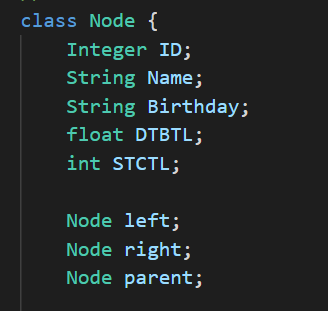
\includegraphics[scale=1.3]{node.png}
    \end{center}
    \caption{Cấu trúc dữ liệu của một node}
    \label{refhinh1}
    \end{figure}
\end{center}

Trong đó:

- ID là mã số sinh viên, thuộc kiểu số nguyên, đóng vai trò là khóa chính của node.

- Name là họ tên của sinh viên đó, thuộc kiểu chuỗi.

- Birthday là ngày tháng năm sinh của sinh viên, thuộc kiểu chuỗi.

- DTBTL là điểm trung bình tích lũy, thuộc kiểu số thực (float).

- STCTL là số tính chỉ tích lũy, thuộc kiểu số nguyên.

- Node left, right, parent là các thành phần khác theo yêu cầu của đề bài.


\newpage
\changefontsizes{14pt}
2. Các giải thuật trên cây. (Hoàn thành 100\%)

a) Cây BST.

o) Giải thuật dựng cây: Dựng cây rỗng, dựng cây với các thông tin ngẫu nhiên, dựng cây lệch trái, dựng cây lệch phải

\begin{center}
    \begin{figure}[htp]
    \begin{center}
     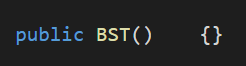
\includegraphics[scale=1.3]{a.png}
    \end{center}
    \caption{Dựng cây rỗng}
    \label{refhinh1}
    \end{figure}
\end{center}
 
\begin{center}
    \begin{figure}[htp]
    \begin{center}
     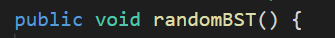
\includegraphics[scale=1.3]{b.png}
    \end{center}
    \caption{Dựng cây với thông tin ngẫu nhiên}
    \label{refhinh1}
    \end{figure}
\end{center}
 
Lệch trái

    \begin{center}
     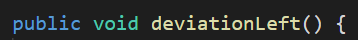
\includegraphics[scale=1.2]{c}
    \end{center}
Lệch phải    
    \begin{center}
     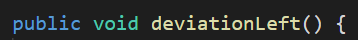
\includegraphics[scale=1.2]{c}
    \end{center}

o Giải thuật duyệt cây theo: LNR, LRN, NLR, RNL, NRL, RLN. Hiển thị đầy đủ thông tin của một node (bao gồm: mã số sinh viên, họ tên, ngày sinh, điểm trung bình, số tín chỉ tích luỹ).

    \begin{center}
     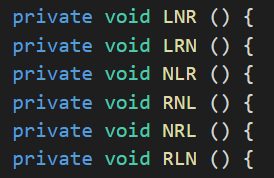
\includegraphics[scale=1.3]{e.png}
    \end{center}

\begin{center}
    \begin{figure}[htp]
    \begin{center}
     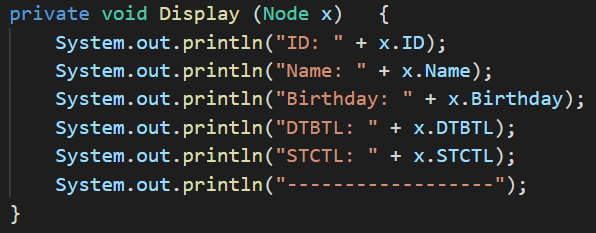
\includegraphics[scale=1]{f.png}
    \end{center}
    \caption{Hiển thị thông tin}
    \label{refhinh1}
    \end{figure}
\end{center}

\newpage
o Giải thuật tìm kiếm: theo mã số sinh viên, theo họ tên, theo ngày sinh, theo điểm trung bình, theo số tín chỉ tích luỹ, tìm phần tử lớn nhất – nhỏ nhất của cây.

    \begin{center}
     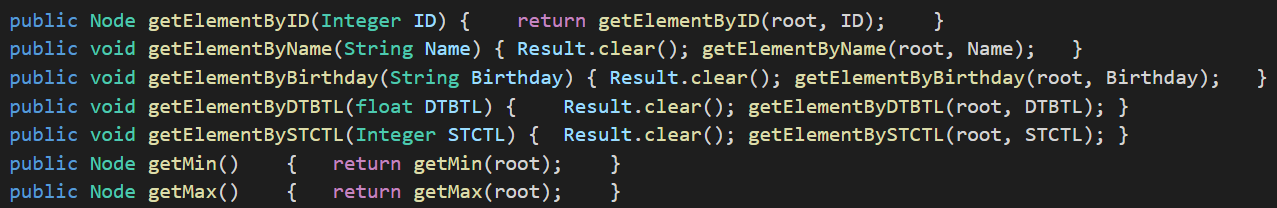
\includegraphics[scale=0.7]{g}
    \end{center}
* Bởi vì khi tìm kiếm theo họ tên, theo ngày sinh, theo điểm trung bình tích lũy, theo số tính chỉ tích lũy không trả về giá trị duy nhất nên kết quả sẽ được lưu vào vector result.
  
\smallskip      
o Giải thuật thêm phần tử vào cây: Thêm tuần tự từng node, thêm danh sách các node.

- Thêm từng node
  \begin{center}
     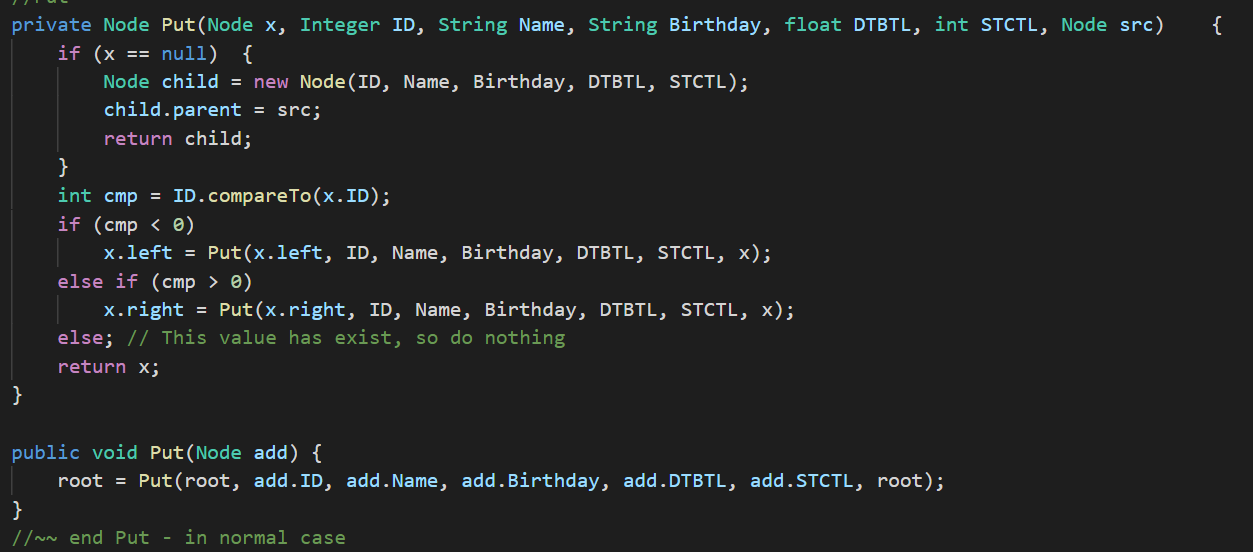
\includegraphics[scale=0.65]{h}
    \end{center}
    
- Thêm danh sách các node
\begin{center}
     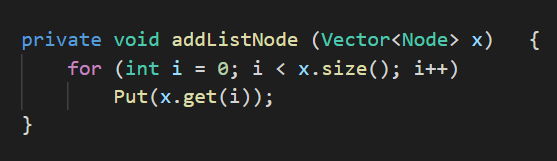
\includegraphics[scale=1]{i}
    \end{center}

o Giải thuật xoá phần tử ra khỏi cây: Xoá tuần tự từng node, xoá danh sách node.

- Xóa từng node
\begin{center}
     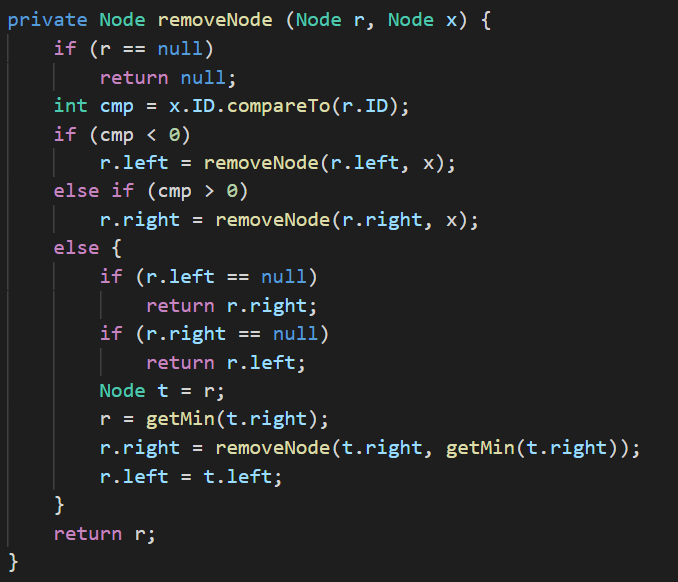
\includegraphics[scale=1]{j}
    \end{center}
- Xóa danh sách các node
\begin{center}
     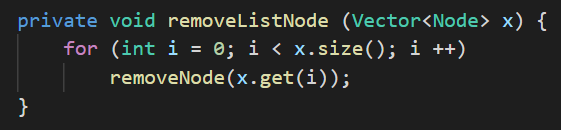
\includegraphics[scale=1]{k}
    \end{center}

o Giải thuật xác định phần tử liền trước (Predecessor), phần tử liền sau (Successor).

- Tìm liền trước
\begin{center}
     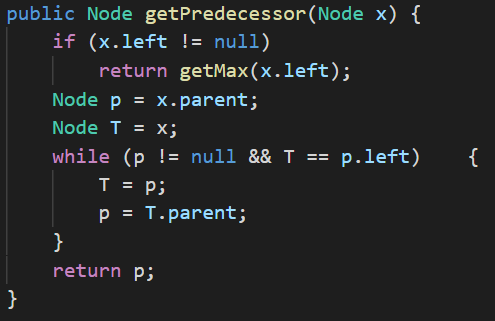
\includegraphics[scale=1]{l}
    \end{center}

- Tìm liền sau
\begin{center}
     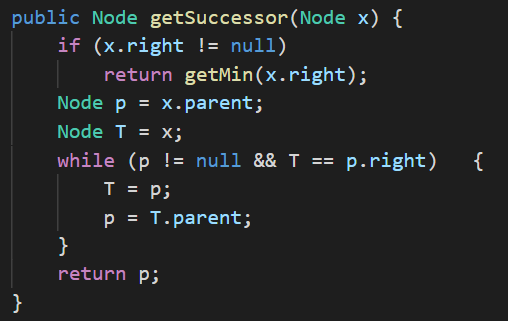
\includegraphics[scale=1]{m}
    \end{center}
    
o Giải thuật cập nhật thông tin trên Node: Cho phép cập nhật họ tên, ngày sinh, điểm trung bình, số tín chỉ dựa vào mã số sinh viên. 
\begin{center}
     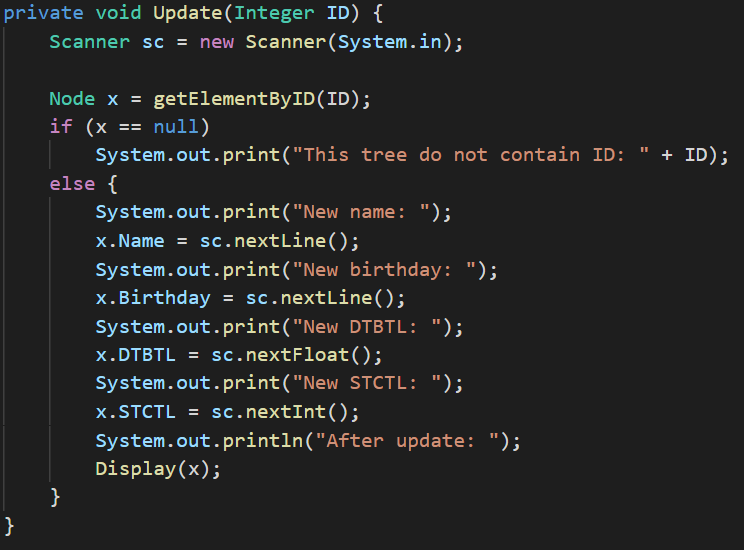
\includegraphics[scale=1]{n}
    \end{center}

\bigskip
b) Cây AVL (tương tự cây BST)
- Tuy nhiên cây AVL không chứa cách dựng cây lệch trái, lệch phải. Ngoài ra cây AVL còn chứa các phương thức kiểm tra và tạo ra cây cân bằng, như:
\begin{center}
     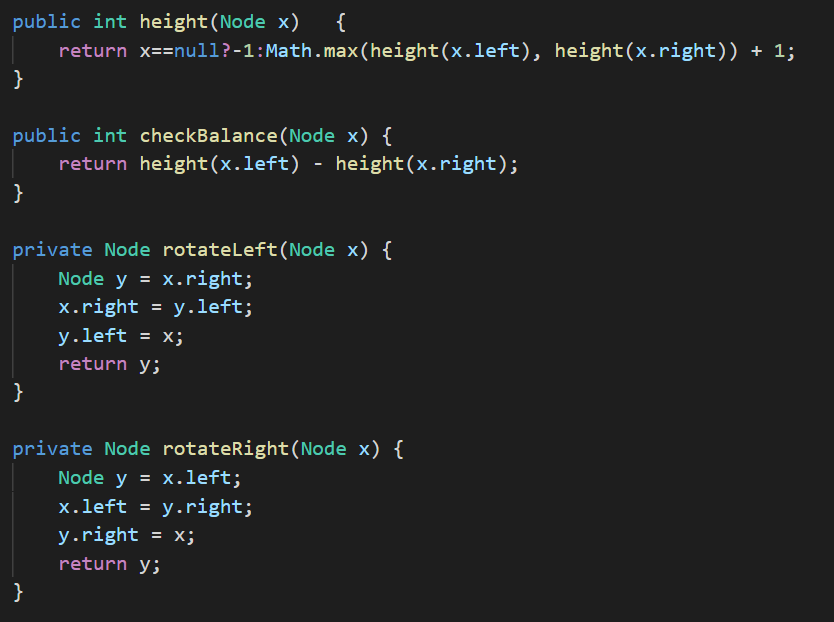
\includegraphics[scale=0.8]{o}
    \end{center}
\begin{center}
     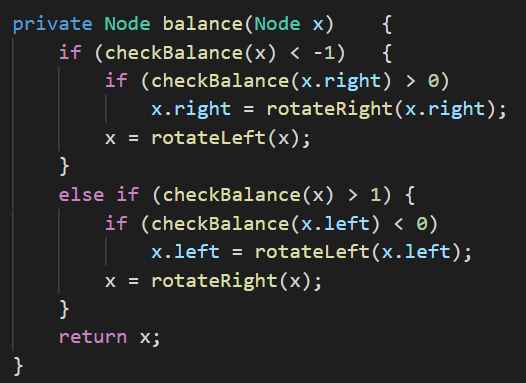
\includegraphics[scale=1]{p}
    \end{center}


\newpage
3. Cách gọi và chạy các phương thức

- Để chạy hàm main, chương trình, dùng lệnh dưới đây trên cửa sổ cmd. Cây BST và cây AVL thực hiện tương tự.

\begin{center}
     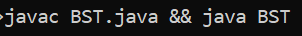
\includegraphics[scale=1]{q}
    \end{center}

Mặc định đọc dữ liệu từ file input.txt (tập tin đi kèm). 

\bigskip
- Kiểm tra các phương thức trong hàm main.

+ Tạo một obj BST để gọi các phương thức (+ Tạo cây rỗng).
\begin{center}
     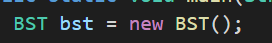
\includegraphics[scale=1]{r}
    \end{center}

+ Đọc dữ liệu từ file input.txt
\begin{center}
     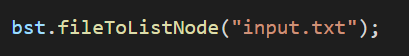
\includegraphics[scale=1]{s}
    \end{center}

+ Tạo cây ngẫu nhiên.
\begin{center}
     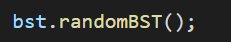
\includegraphics[scale=1]{t}
    \end{center}

+ Tạo cây lệch trái.
\begin{center}
     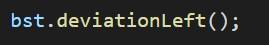
\includegraphics[scale=1]{u}
    \end{center}

+ Tạo cây lệch phải.
\begin{center}
     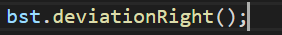
\includegraphics[scale=1]{v}
    \end{center}

+ Các hàm duyệt cây.
\begin{center}
     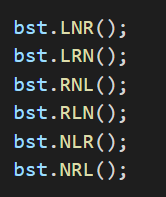
\includegraphics[scale=1.2]{w}
    \end{center}

+ Tìm kiếm dựa vào ID. Trong trường hợp này, ID là 10.
\begin{center}
     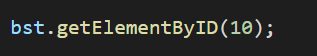
\includegraphics[scale=1.2]{x}
    \end{center}

+ Tìm kiếm dựa vào Tên.
\begin{center}
     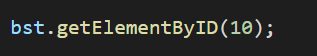
\includegraphics[scale=1.2]{x}
    \end{center}
+ Tìm kiếm dựa vào birthday
\begin{center}
     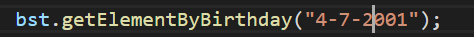
\includegraphics[scale=1.2]{y}
    \end{center}
+ Tìm kiếm dựa vào Điểm trung bình tích lũy.
\begin{center}
     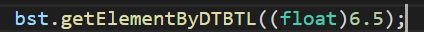
\includegraphics[scale=1.2]{z}
    \end{center}
+ Tìm kiếm dựa vào số tính chỉ tích lũy
\begin{center}
     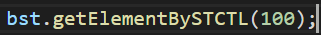
\includegraphics[scale=1.2]{a1}
    \end{center}
+ Tìm min và max
\begin{center}
     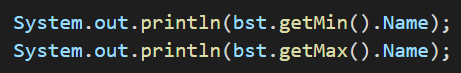
\includegraphics[scale=1.2]{a2}
    \end{center}

+ Chèn một danh sách các node
\begin{center}
     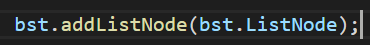
\includegraphics[scale=1.2]{a3}
    \end{center}

+ Xóa một node, trong trường hợp này là node có ID = 9
\begin{center}
     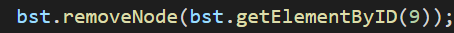
\includegraphics[scale=1.2]{a4}
    \end{center}

+ Xóa danh sách các node
\begin{center}
     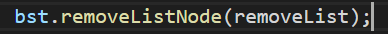
\includegraphics[scale=1.2]{a5}
    \end{center}

+ Tìm liền trước và liền sau, trong trường họp này là liền trước và liền sau của phần tử có ID = 59
\begin{center}
     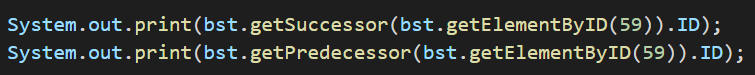
\includegraphics[scale=1.2]{a6}
    \end{center}
    
+ Cập nhật 1 phần từ, trong trường hợp này là phần tử có ID = 10
\begin{center}
     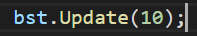
\includegraphics[scale=1.2]{a7}
    \end{center}
    
4. Hiện thực trực quan hóa (Chưa hoàn thành)
    



    

    
    


%Page ?? + 1
\newpage
\changefontsizes{16pt}
\centerline{\textbf{TÀI LIỆU THAM KHẢO}}

\vspace{1.2cm}
\changefontsizes{14pt}
\textbf{Tiếng Việt}


\vspace{3cm}
\textbf{Tiếng Anh}



\end{document}